\documentclass[aspectratio=169]{beamer}
% \setbeamertemplate{footline}[frame number]
\usepackage{color,amsmath}
\usepackage{subfigure}
\usepackage{booktabs}
\usepackage{framed}
\usepackage{comment}
\hypersetup{
colorlinks=true,
linkcolor=blue,
filecolor=magenta,      
urlcolor=blue,
pdftitle={Overleaf Example},
pdfpagemode=FullScreen}
\usepackage{tabularx}

%%%%%%%%%%%%%%%%%%%%%%%%%%
\title[]{Survey research in the digital age}
\author[]{Bernhard Clemm von Hohenberg\\Department of Computational Social Science\\GESIS}
\date[]{Summer Institutes in Computational Social Science\\July 28, 2023}
\begin{document}
%%%%%%%%%%%%%%%%%%%%%%%%%%
\frame{\titlepage}
%%%%%%%%%%%%%%%%%%%%%%%%%%
\begin{frame}{Schedule}

\vspace{0.5em}
\begin{itemize}
\item 9.00-9.45 Introduction \& total error survey framework
\item 9.45-10.15 Probability and non-probability sampling
\vspace{0.5em}
\item Coffee break
\vspace{0.5em}
\item \textcolor{violet}{10.30-11.00 Computer-administered interviewing}
\item 11.00-11.30 Linking surveys to big data
\item 11:30-13:00 Intro and begin group exercise
\vspace{0.5em}
\item Lunch (or Eisbach plunge)
\vspace{0.5em}
\item 14:00-15:45 Continue group exercise
\end{itemize}

\end{frame}
%%%%%%%%%%%%%%%%%%%%%%%%%%%
\begin{frame}{Credits}

These materials build heavily on Matthew Salganik's 2019 SICSS class as well as Chapter 3 of ``Bit by Bit: Social Research in the Digital Age''.

\end{frame}
%%%%%%%%%%%%%%%%%%%%%%%%%%%
\begin{frame}
\begin{center}
\renewcommand{\arraystretch}{1.5}
\begin{tabular}{p{0.1\textwidth}p{0.26\textwidth}p{0.24\textwidth}p{0.24\textwidth}}
& \textbf{Sampling} & \textbf{Interviews} & \textbf{Data environment}\\
\hline \hline
1st era & Area probability & Face-to-face & Stand-alone \\
\hline
2nd era & Random digital dial probability & Telephone & Stand-alone \\
\hline
3rd era & Non-probability & \textcolor{violet}{Computer-administered} & Linked \\
\end{tabular}
\end{center}

\end{frame}
%%%%%%%%%%%%%%%%%%%%%%%%%%%
\begin{frame}{Warm-up exercise}

Go to \url{https://tinyurl.com/xv26a3s7} and do the questionnaire.

\end{frame}
%%%%%%%%%%%%%%%%%%%%%%%%%%%
\begin{frame}{Warm-up exercise}

\begin{center}
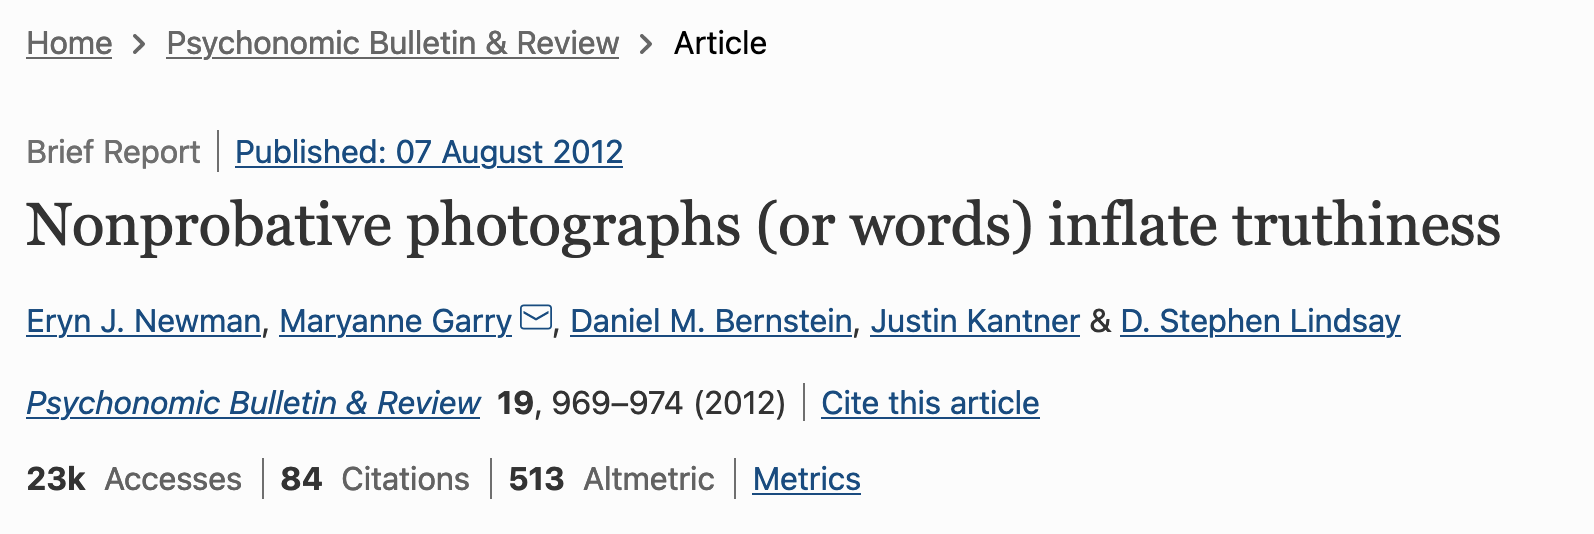
\includegraphics[width=\textwidth]{figures/newman2012-abstract.png}
\end{center}

\vfill
\TINY{\url{https://link.springer.com/article/10.3758/s13423-012-0292-0}}

\end{frame}
%%%%%%%%%%%%%%%%%%%%%%%%%%%
\begin{frame}{Warm-up exercise}

Rating general knowledge statements for their truth, either with or without image:

\vfill

\begin{column}{0.45\textwidth}
\begin{center}
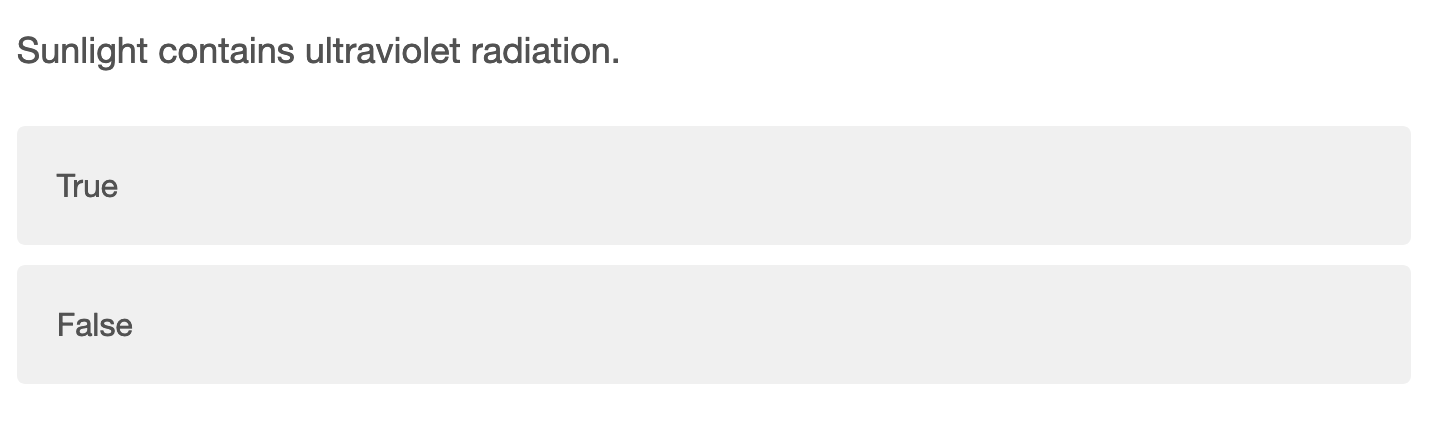
\includegraphics[width=\textwidth]{figures/warmup2-control.png}
\end{center}
\end{column}
\pause
\begin{column}{0.45\textwidth}
\begin{center}
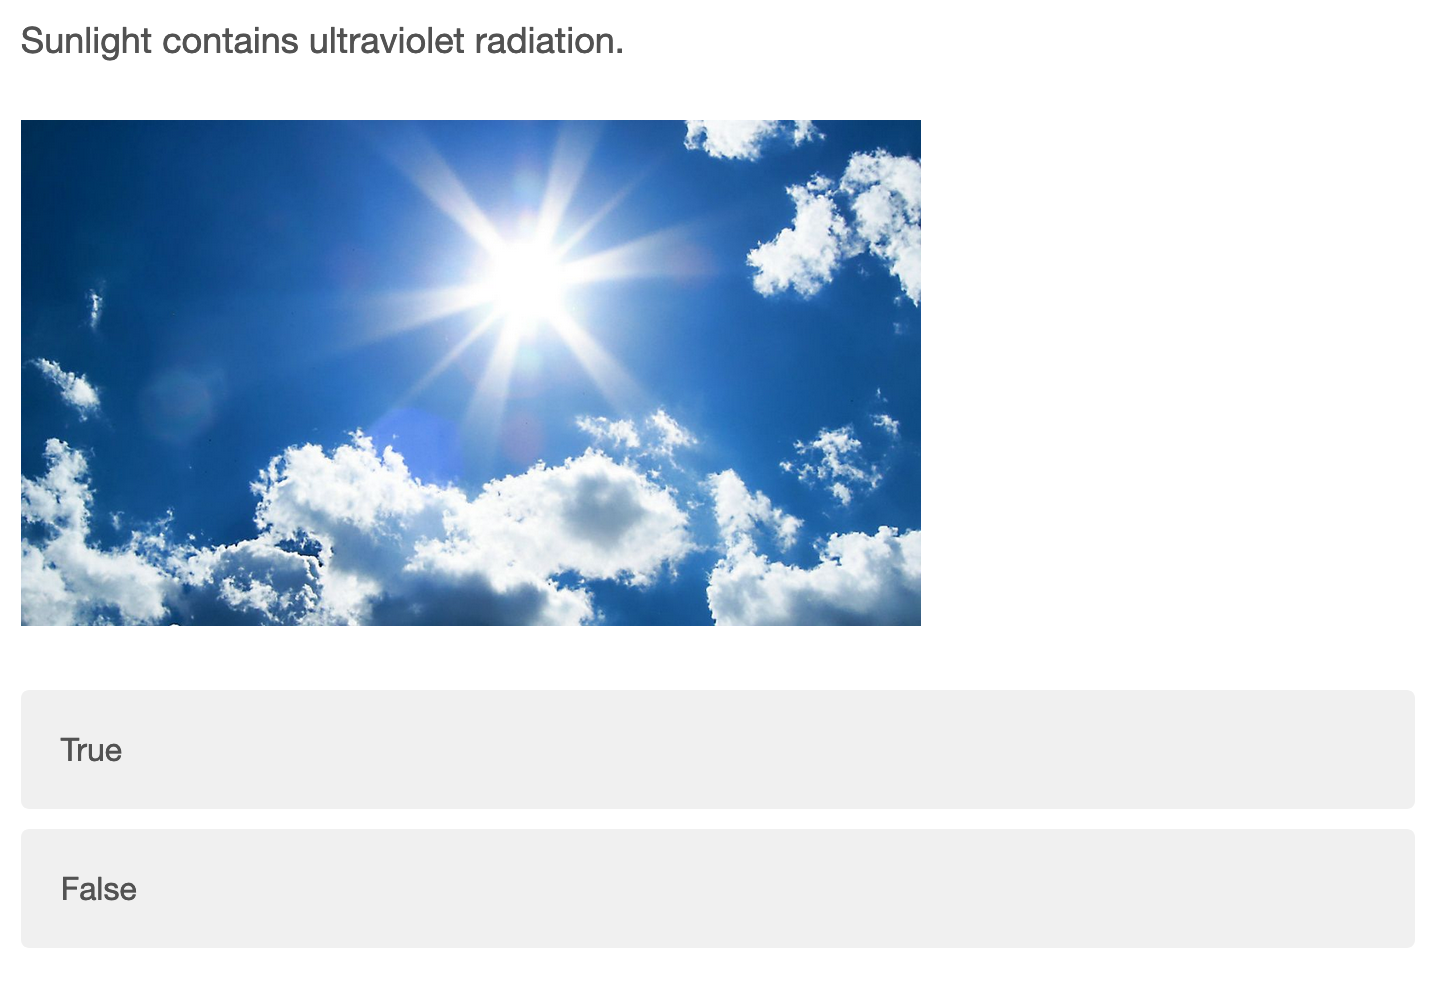
\includegraphics[width=\textwidth]{figures/warmup2-treatment.png}
\end{center}
\end{column}

\end{frame}
%%%%%%%%%%%%%%%%%%%%%%%%%%%
\begin{frame}

\begin{center}
\LARGE Ways in which we can---and need to---ask questions have changed
\end{center}

\end{frame}
%%%%%%%%%%%%%%%%%%%%%%%%%%%
\begin{frame}{New ways to ask}

Ways in which we need to ask differently:

\begin{itemize}
    \item Questions look and work differently on digital vs. analogue, and between digital devices (\textbf{mode effects})
\end{itemize}
\pause

Ways in which we can ask differently:

\begin{itemize}
    \item Online questionnaires allow embedding multimedia content (previous example)
    \pause
    \item Shift to mobiles allow asking question at higher frequency and at targeted times (\textbf{momentary assessments})
    \pause
    \item Apps can make research questions more motivating (\textbf{gamification})
    \pause
    \item Software allows updating questionnaires on the fly (\textbf{adaptive experimentation}) 
\end{itemize}


\end{frame}
%%%%%%%%%%%%%%%%%%%%%%%%%%%
\begin{frame}{Mode effects}

Asking questions digitally requires respecting digital setup and type of device, for example:

\begin{itemize}
    \item ``Primacy effect'' found to be larger on mobile
    \item Online respondents are more impatient
    \item Some classic response formats do not work on mobile (e.g., question matrix)
\end{itemize}

\end{frame}
%%%%%%%%%%%%%%%%%%%%%%%%%%%
\begin{frame}

\begin{column}{0.45\textwidth}
\begin{center}
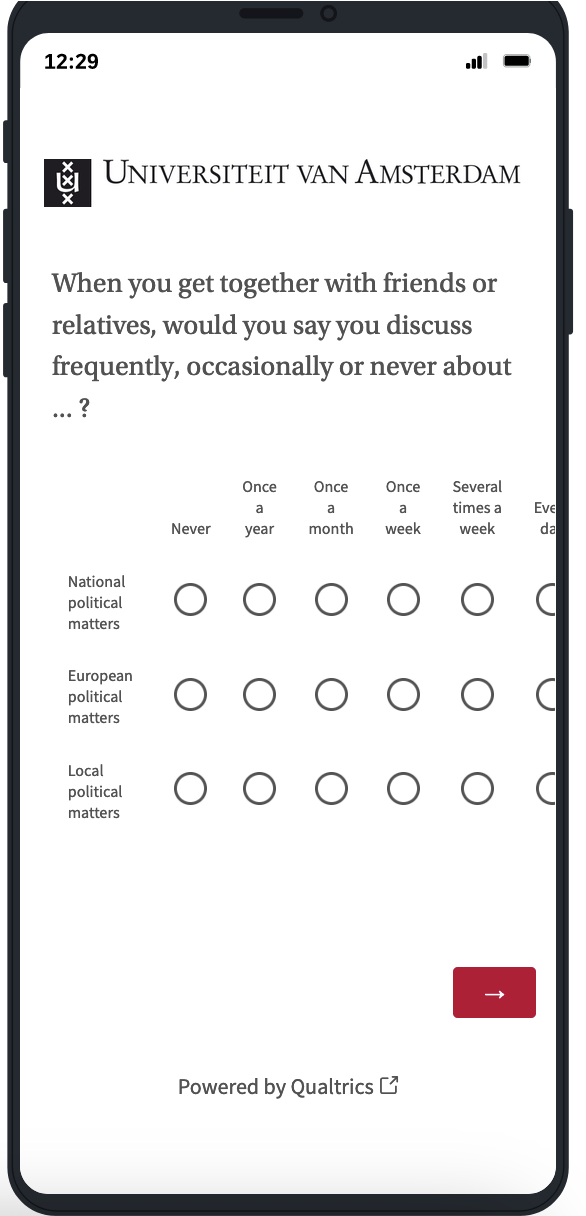
\includegraphics[width=0.55\textwidth]{figures/mobile-matrix.png}
\end{center}
\end{column}
\begin{column}{0.45\textwidth}
\begin{center}
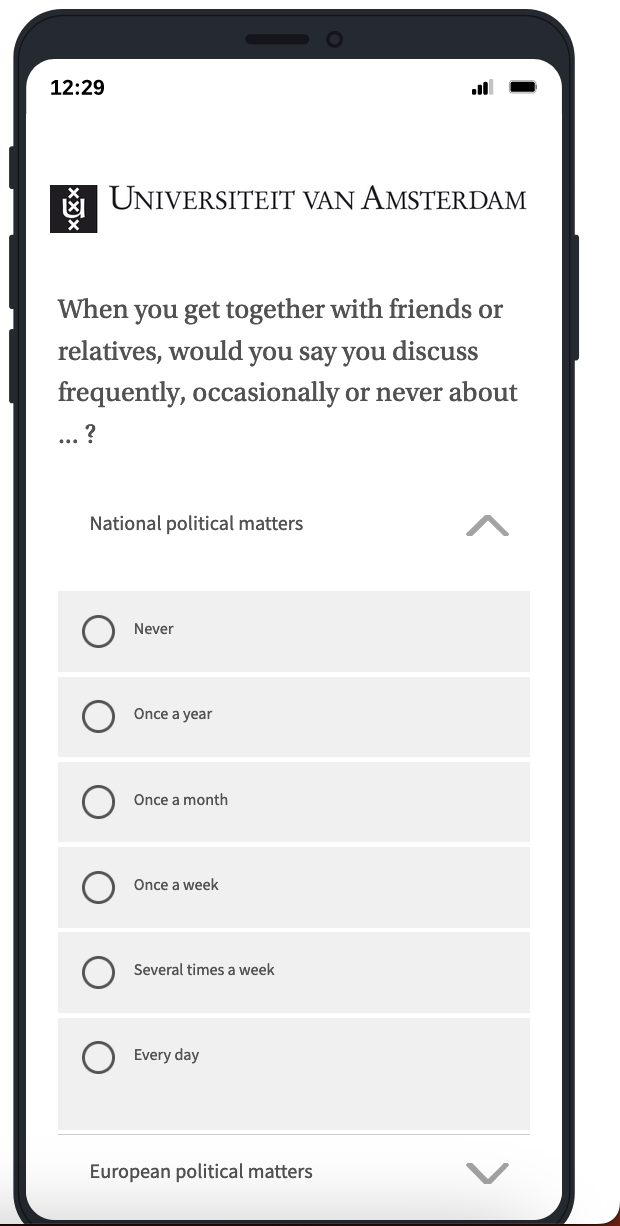
\includegraphics[width=0.6\textwidth]{figures/mobile-list.png}
\end{center}
\end{column}


\end{frame}
%%%%%%%%%%%%%%%%%%%%%%%%%%%
\begin{frame}{Momentary assessments}

Ecological momentary assessment (experience sampling)

\begin{itemize}
    \item Collection of data in real-world environments
    \item Focus on individuals’ current or very recent states or behaviors
    \item May be event-based, time-based, or randomly prompted
    \item Completion of multiple assessments over time
\end{itemize}

\end{frame}
%%%%%%%%%%%%%%%%%%%%%%%%%%%
\begin{frame}

\begin{center}
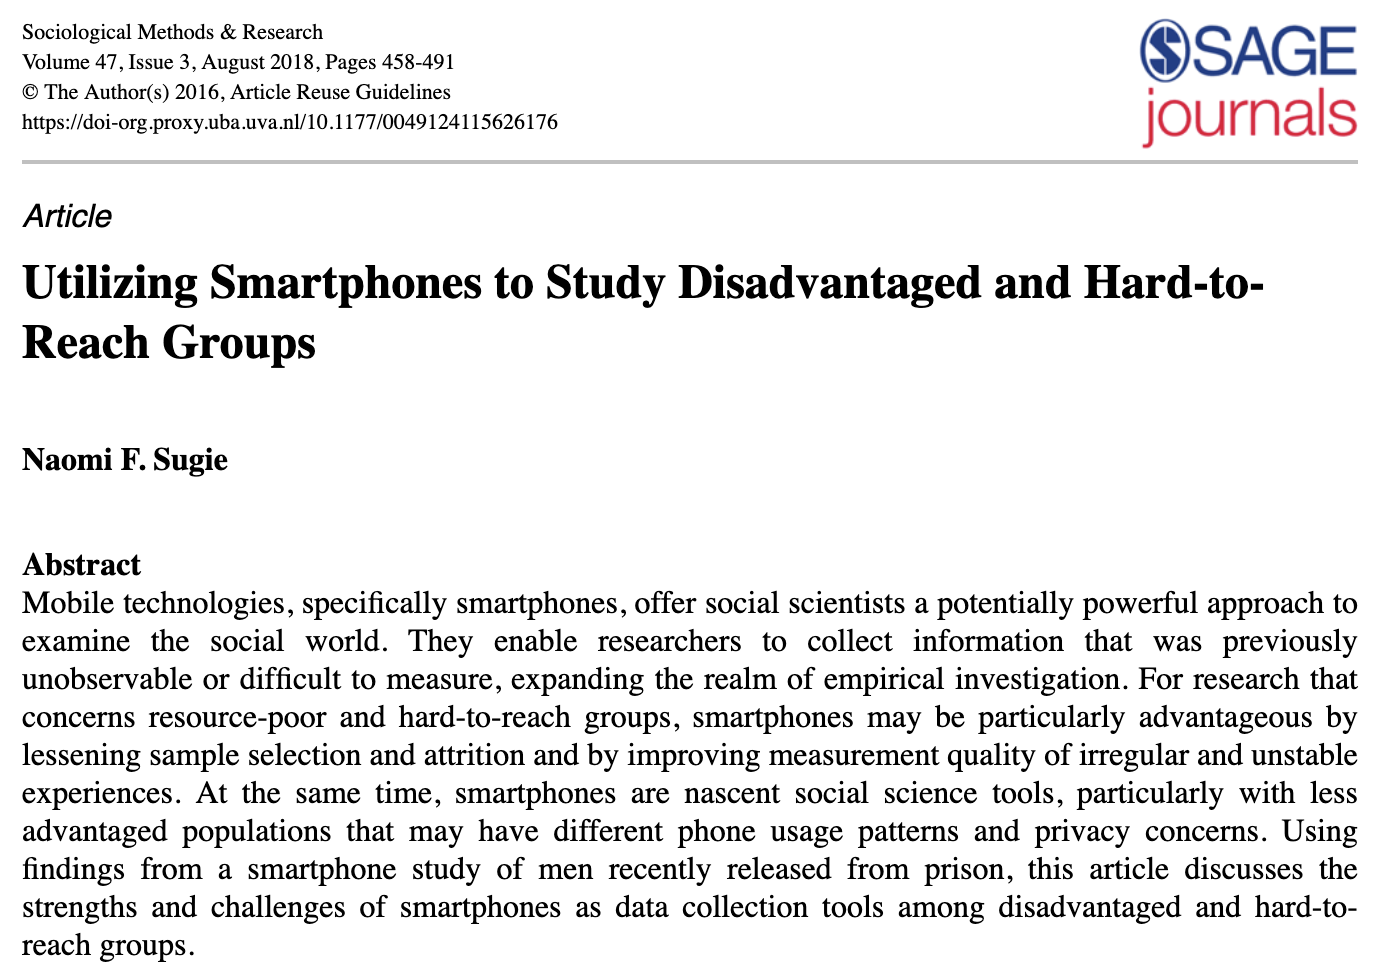
\includegraphics[width=0.65\textwidth]{figures/sugie2016-abstract.png}
\end{center}

\vfill
\TINY{\url{https://doi.org/10.1177/00491241156261769}}


\end{frame}
%%%%%%%%%%%%%%%%%%%%%%%%%%%
\begin{frame}

\begin{center}
Questions
\end{center}

\end{frame}
%%%%%%%%%%%%%%%%%%%%%%%%%%%

\end{document}
